\chapter{Entwurf und Implementierung}\label{sec:impl}

Hier wird die eigene Lösung des Problems vorgestellt,
sowie interessante Details der Implementierung.
Was also wurde praktisch in dieser Arbeit geleistet?

\begin{figure}
	\centering

	\hfill
	\subfloat[Original data flow graph]{\label{fig:innerSCCDataFlow}
	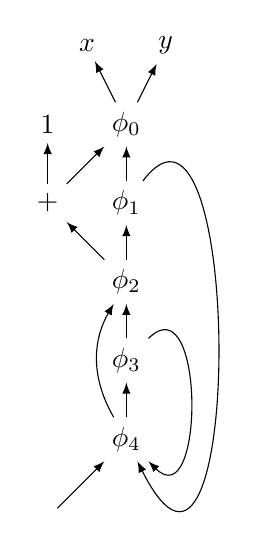
\begin{tikzpicture}
		\path
			  ( 0,   0) node (other)  {$\phi_0$}
			 +(-0.5, 1) node (x)      {$x$}
			 +( 0.5, 1) node (y)      {$y$}
			 +(-1,   0) node (one)    {$1$}
			++( 0,  -1) node (outer1) {$\phi_1$}
			++( 0,  -1) node (outer2) {$\phi_2$}
			 +(-1,   1) node (plus)   {$+$}
			++( 0,  -1) node (inner1) {$\phi_3$}
			++( 0,  -1) node (inner2) {$\phi_4$}
			 +(-1,  -1) node (use)    {}
		;
		\node at (1.2,0) {};
		\draw[-latex]         (other)  -> (x);
		\draw[-latex]         (other)  -> (y);
		\draw[-latex]         (plus)   -> (one);
		\draw[-latex]         (plus)   -> (other);
		\draw[-latex,overlay] (outer1) .. controls (1.5,1) and (1.5,-7) .. (inner2);
		\draw[-latex]         (outer1) -> (other);
		\draw[-latex]         (outer2) -> (outer1);
		\draw[-latex]         (outer2) -> (plus);
		\draw[-latex]         (inner1) -> (outer2);
		\draw[-latex,overlay] (inner1) .. controls (1,-2) and (1,-5) .. (inner2);
		\draw[-latex]         (inner2) edge[bend left] (outer2);
		\draw[-latex]         (inner2) -> (inner1);
		\draw[-latex]         (use)    -> (inner2);
	\end{tikzpicture}
	}
	\hfill
	\subfloat[SCCs and their operands]{\label{fig:innerSCCSCCs}
	\begin{tikzpicture}
		\path
			  ( 0,   0) node (other)  {$\phi_0$}
			 +(-0.5, 1) node (x)      {$x$}
			 +( 0.5, 1) node (y)      {$y$}
			++( 0,  -1) node (outer1) {$\phi_1$}
			++( 0,  -1) node (outer2) {$\phi_2$}
			 +(-1,   1) node (plus)   {$+$}
			++( 0,  -1) node (inner1) {$\phi_3$}
			++( 0,  -1) node (inner2) {$\phi_4$}
			 +(-1,  -1) node (use)    {}
		;
		\node at (1.2,0) {};
		\draw[-latex,dashed]  (other)  -> (x);
		\draw[-latex,dashed]  (other)  -> (y);
		\draw[-latex,overlay] (outer1) .. controls (1.5,1) and (1.5,-7) .. (inner2);
		\draw[-latex,dashed]  (outer1) -> (other);
		\draw[-latex]         (outer2) -> (outer1);
		\draw[-latex,dashed]  (outer2) -> (plus);
		\draw[-latex]         (inner1) -> (outer2);
		\draw[-latex,overlay] (inner1) .. controls (1,-2) and (1,-5) .. (inner2);
		\draw[-latex]         (inner2) edge[bend left] (outer2);
		\draw[-latex]         (inner2) -> (inner1);

		\begin{pgfonlayer}{background}
			\tikzselect{1}{
				(other.west) (other.north) (other.east) (other.south)
			}
			\tikzselect{0.3}{
				(outer1.west) (outer1.north) (outer1.east)
				(inner2.east) (inner2.south) (inner2.west)
			}
		\end{pgfonlayer}
	\end{tikzpicture}
	}
	\hfill
	\subfloat[Inner SCC]{\label{fig:innerSCCinnerSCC}
	\begin{tikzpicture}
		\path
			  (0, 0) node (outer1) {}
			++(0,-1) node (outer2) {$\phi_2$}
			++(0,-1) node (inner1) {$\phi_3$}
			++(0,-1) node (inner2) {$\phi_4$}
			 +(0,-1) node (use)    {}
		;
		\node at (0.8,0) {};
		\draw[-latex,overlay] (inner1) .. controls (1,-1) and (1,-4) .. (inner2);
		\draw[-latex,dashed]  (inner1) -> (outer2);
		\draw[-latex]         (inner2) -> (inner1);
		\draw[-latex,dashed]  (inner2) edge[bend left] (outer2);

		\begin{pgfonlayer}{background}
			\tikzselect{0.6}{
				(inner1.west) (inner1.north) (inner1.east)
				(inner2.east) (inner2.south) (inner2.west)
			}
		\end{pgfonlayer}
	\end{tikzpicture}
	}
	\hfill
	\subfloat[Optimized data flow graph]{\label{fig:innerSCCoptimized}
	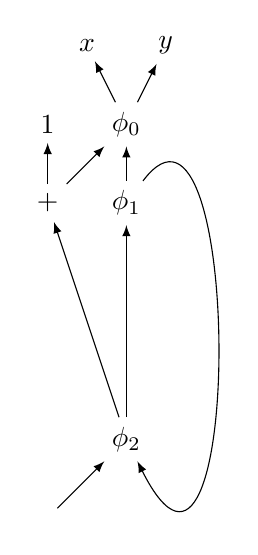
\begin{tikzpicture}
		\path
			  ( 0,   0) node (other)  {$\phi_0$}
			 +(-0.5, 1) node (x)      {$x$}
			 +( 0.5, 1) node (y)      {$y$}
			 +(-1,   0) node (one)    {$1$}
			++( 0,  -1) node (outer1) {$\phi_1$}
			 +(-1,   0) node (plus)   {$+$}
			++( 0,  -3) node (outer2) {$\phi_2$}
			 +(-1,  -1) node (use)    {}
		;
		\node at (1.2,0) {};
		\draw[-latex]         (other)  -> (x);
		\draw[-latex]         (other)  -> (y);
		\draw[-latex]         (plus)   -> (one);
		\draw[-latex]         (plus)   -> (other);
		\draw[-latex,overlay] (outer1) .. controls (1.5,1) and (1.5,-7) .. (outer2);
		\draw[-latex]         (outer1) -> (other);
		\draw[-latex]         (outer2) -> (outer1);
		\draw[-latex]         (outer2) -> (plus);
		\draw[-latex]         (use)    -> (outer2);
	\end{tikzpicture}
	}
	\hfill
	\caption{Some algorithm~\cite{braun13cc} detects the inner SCC spanned by $\phi_3$ and $\phi_4$. This SCC represents the same value. Thus, it gets replaced by $\phi_2$.}
\label{fig:optimizations}
\end{figure}


Für eigene Grafiken und Diagramme empfehlen wir TikZ
(TikZ ist kein Zeichenprogramm).
Damit kann man innerhalb von \TeX Dokumenten Zeichenoperationen angeben.
Im Gegensatz zu externen Grafiken,
die per png/jpg/pdf eingebunden werden,
passt mit TikZ die Schrift exakt zum restlichen Dokument.
Zwar ist die Einarbeitung schwieriger,
aber die Qualität ist kaum zu überbieten.
Ein Beispiel aus einem unserer Paper~\cite{braun13cc}
siehst du in \cref{fig:optimizations}.

\begin{figure}
\centering
\begin{tikzpicture}[scale=1.0, transform shape]
	\node[graph]{
		\begin{tikzpicture}[remember picture]
			\node[block] (startblock) {
				\begin{tikzpicture}
					\node[start]   (start)      at ( 0,5) {Start};
					\node[memory]  (initialMem) at (-2,4) {Mem};
					\node[proj]    (args)       at ( 0,4) {Args};
					\node[proj]    (arg0)       at (-1,3) {Arg 0};
					\node[proj]    (arg1)       at ( 1,3) {Arg 1};
					\node[firm]    (cmp)        at ( 0,2) {Cmp};
					\node[control] (cond)       at ( 0,1) {Cond};
					\node[control] (false)      at (-1,0) {False};
					\node[control] (true)       at ( 1,0) {True};

					\draw[memoryDependency]  (initialMem)  -- ++(0,0.5) -| (start.240);
					\draw[dataDependency]    (args)        --              (start);
					\draw[dataDependency]    (arg0.north)  -- ++(0,0.1) -| (args.240);
					\draw[dataDependency]    (arg1.north)  -- ++(0,0.1) -| (args.300);
					\draw[dataDependency]    (cmp.120)     -- ++(0,0.1) -| (arg0);
					\draw[dataDependency]    (cmp.60)      -- ++(0,0.1) -| (arg1);
					\draw[dataDependency]    (cond)        --              (cmp);
					\draw[controlDependency] (false.north) -- ++(0,0.1) -| (cond.240);
					\draw[controlDependency] (true.north)  -- ++(0,0.1) -| (cond.300);
				\end{tikzpicture}
			};
			\node[block, anchor=north east] (left) at ($(startblock.south) + (-1,-0.5)$) {
				\begin{tikzpicture}
					\node[const] (c0) at (0,0) {Const 0};
				\end{tikzpicture}
			};
			\node[block, anchor=north west] (right) at ($(startblock.south) + (1,-0.5)$) {
				\begin{tikzpicture}
					\node[const] (c1) at (0,0) {Const 1};
				\end{tikzpicture}
			};
			\node[block, anchor=north] (end) at ($(left.south east)!0.5!(right.south west) + (0,-0.5)$) {
				\begin{tikzpicture}
					\node[phi]     (phi) at (0,2) {Phi};
					\node[firm]    (add) at (0,1) {Add};
					\node[control] (ret) at (0,0) {Return};

					\draw[dataDependency] (add.120) -- (phi.240);
					\draw[dataDependency] (add.60)  -- (phi.300);
					\draw[dataDependency] (ret)     -- (add);
				\end{tikzpicture}
			};

			% Data dependencies
			\begin{scope}[every path/.style = {dataDependency}]
				\draw (phi.120) -- +(0,0.5) -| (c0.300);
				\draw (phi.60)  -- +(0,0.5) -| (c1.240);
			\end{scope}

			% Control dependencies
			\begin{scope}[every path/.style = {controlDependency}]
				\draw (left.north)  -- ++(0,0.2) -| (false);
				\draw (right.north) -- ++(0,0.2) -| (true);
				\draw (end.110) -- ++(0,0.2) -| (left.south);
				\draw (end.70) -- ++(0,0.2) -| (right.south);
			\end{scope}

			% Memory dependencies
			\begin{scope}[every path/.style = {memoryDependency}]
				\draw (ret.120) -- ++(0,0.2) -- ++(-3,0) -- ++(0,6) -| (initialMem);
			\end{scope}
		\end{tikzpicture}
	};
\end{tikzpicture}
\caption{Ein Firm-Graph einer Funktion,
der zwei Eingabewerte (Arg 0 und Arg 1) vergleicht (Cmp+Cond) und
0 oder 1 als Wert erzeugt.
Zurückgegeben (Return) wird der erzeugte Wert addiert (Add) mit sich selbst.}
\label{fig:firm}
\end{figure}


Für Firm-Graphen die bei uns im Compilerbau häufig vorkommen,
haben wir ein extra TiKZ Paket gebaut.
Dieses erleichtert das Zeichnen von Graphen,
die wie yComp aussehen.
\Cref{fig:firm} zeigt ein Beispiel.

